\documentclass{beamer}

\usepackage{Haust2016glærur}

\title{Stærðfræðimynstur í tölvunarfræði}
\subtitle{Vika 1, seinni fyrirlestur}

\begin{document}

\begin{frame}
\titlepage
\end{frame}

\section{Inngangur}

\begin{frame}{Í síðasta tíma}
\begin{itemize}
 \item Kynntumst hugtakinu um \emph{yrðingar}
 \begin{itemize}
  \item Yrðingar eru fullyrðingar sem eru áreiðanlega sannar eða áreiðanlega ósannar
  \item Yrðingar má tákna með rökbreytum
 \end{itemize}
 \item Sáum rökvirkja sem vinna á yrðingum, sanntöflur, skilgreiningu á jafngildi yrðinga
\end{itemize}
\end{frame}

\section{Hagnýting yrðinga}

\subsection{Forritun}

\begin{frame}[fragile]{Í forritun}
\begin{columns}
\column{0.4\textwidth}
\begin{itemize}
 \item Ýmis form yrðinga koma fyrir í öllum forritunarmálum (sem kennari hefur séð)
 \item Fáið að sjá á næstu vikum í Tölvunarfræði 1 og Tölvunarfræði 1a!
\end{itemize}
\column{0.6\textwidth}
\begin{minted}[fontsize=\scriptsize, frame=lines, label=Yrðingar í Java]{java}
public static void main(String []args) {
  Boolean p = true;
  Boolean q = false;
  // p && q þýðir ``p og q''
  System.out.println(p && q);
  // p || q þýðir ``p eða q''
  System.out.println(p || q);
}
\end{minted}

\end{columns}
\end{frame}

\subsection{Gátur}

\begin{frame}{Lausnir á gátum}
\begin{itemize}
 \item Ýmsar gátur má leysa með því að setja þær fram á yrðingaformi
 \item Brjótum setningar gátunnar niður í yrðingar
 \item Könnum sanngildi yrðinganna
\end{itemize}
\end{frame}

\begin{frame}{Riddarar og ribbaldar}
\begin{itemize}
 \item Við erum stödd á eyju þar sem íbúar eru annaðhvort riddarar eða ribbaldar\pause
 \begin{itemize}
  \item Riddarar segja alltaf satt
  \item Ribbaldar segja alltaf ósatt
 \end{itemize}
 \item Hittum tvo einstaklinga, $A$ og $B$. 
 \begin{itemize}
  \item $A$ segir: ``$B$ er riddari.''
  \item $B$ segir: ``Við erum af mismunandi gerðum.''
 \end{itemize}
 \item Af hvaða gerðum eru $A$ og $B$?
\end{itemize}
\end{frame}

\begin{frame}{Riddarar og ribbaldar á yrðingaformi}
\begin{itemize}
 \item Látum $p$ vera yrðinguna ``$A$ er riddari''
 \item Látum $q$ vera yrðinguna ``$B$ er riddari''
 \item Hvað getum við fullyrt út frá því sem $A$ sagði? \pause
 \begin{itemize}
  \item Ef $p$ er satt, þá er $q$ satt
  \item Ef $q$ er ósatt, þá er $p$ ósatt
 \end{itemize}
 \item Hvað getum við fullyrt út frá því sem $B$ sagði? \pause
 \begin{itemize}
  \item Ef $p \oplus q$ er satt, þá er $q$ satt
  \item Ef $p \oplus q$ er ósatt, þá er $q$ ósatt
 \end{itemize}
 \item Hvert er sanngildi $(p \leftrightarrow q) \land ((p \oplus q) \leftrightarrow q)$?
\end{itemize}
\end{frame}

\begin{frame}{Riddarar og ribbaldar - sanntafla}
Komumst að sanngildi $(p \leftrightarrow q) \land ((p \oplus q) \leftrightarrow q)$ með sanntöflu:
\begin{center}
\begin{tabular}{ccccc}
\toprule
$p$&$q$&$p \leftrightarrow q$&$p \oplus q$& $(p \oplus q) \leftrightarrow q$\\
\midrule
0&0&1&0&1\\
1&0&0&1&0\\
0&1&0&1&1\\
1&1&1&0&0\\
\bottomrule
\end{tabular}
\end{center}\pause
Fullyrðingarnar standast einungis þegar bæði $A$ og $B$ eru ribbaldar.
\end{frame}

\subsection{Rökrásir}

\begin{frame}{Rökrásir}
\begin{itemize}
 \item Stafrænar rásir eru byggðar upp eins og yrðingar
 \item Notum sanngildin $0$ og $1$ sem ``merki''
 \item Búum til rafrás sem tekur við merkjum $p_1, p_2, \ldots, p_n$ og skilar merkjum $s_1, s_2, \ldots s_n$
 
 \item Notum rökhlið (e. \emph{logic gates}) til að breyta merkjunum
\end{itemize}
\end{frame}

\begin{frame}{Rökrásir}
Getum við búið til rökrás sem táknar yrðinguna $(p \land \lnot q) \lor \lnot r$ með því að nota þessi grunnhlið?
\begin{center}
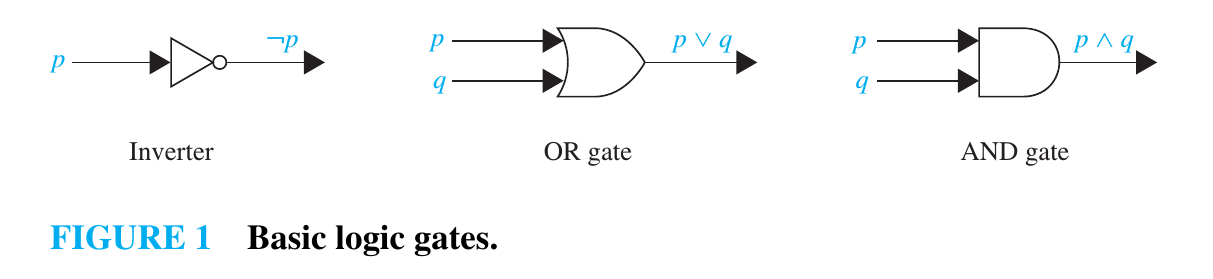
\includegraphics[width=0.8\textwidth]{logic-circuit}\\
\pause
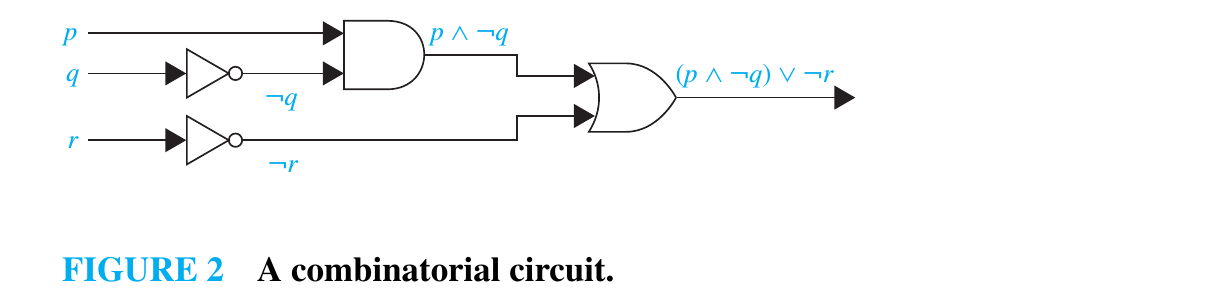
\includegraphics[width=0.8\textwidth]{comi-circuit}
\end{center}
Mynd úr kafla 1.2 í bók
\end{frame}

\section{Jafngildi yrðinga}

\begin{frame}{Jafngildi}
Í síðasta tíma sáum við skilgreiningu á jafngildi:

\begin{tcolorbox}[title=Jafngildi]
Yrðingarnar $p$ og $q$ eru jafngildar (e. \emph{equivalent}) sé $p \leftrightarrow q$ sísanna.
\end{tcolorbox}

Við munum tákna jafngildi með $\equiv$.
\end{frame}

\begin{frame}{De Morgan jafngildin}
Mikilvæg jafngildi sem oft koma upp eru jafngildi/reglur De Morgans, sem eru eftirfarandi:

\[
 \lnot ( p \land q ) \equiv \lnot p \lor \lnot q
\]

\[
 \lnot (p \lor q ) \equiv \lnot p \land \lnot q
\]

\end{frame}

\begin{frame}{De Morgan og sanntöflur}
Sýnum fram á að $\lnot (p \lor q ) \equiv \lnot p \land \lnot q$ með sanntöflu:
\begin{center}
\begin{tabular}{ccccccc}
\toprule
$p$&$q$&$p \lor q$&$\lnot(p \lor q)$&$\lnot p$&$\lnot q$&$\lnot p \land \lnot q$\\
\midrule
0&0&0&1&1&1&1\\
1&0&1&0&0&1&0\\
0&1&1&0&1&0&0\\
1&1&1&0&0&0&0\\
\bottomrule
\end{tabular}
\end{center}
$\lnot (p \lor q ) \leftrightarrow \lnot p \land \lnot q$ er sísanna, svo reglan gildir.
\end{frame}

\subsection{Ýmis jafngildi}

\begin{frame}{Ýmis jafngildi}
\begin{columns}
\column{0.25\textwidth}
Tafla úr kafla 1.3
\column{0.75\textwidth}
\begin{center}
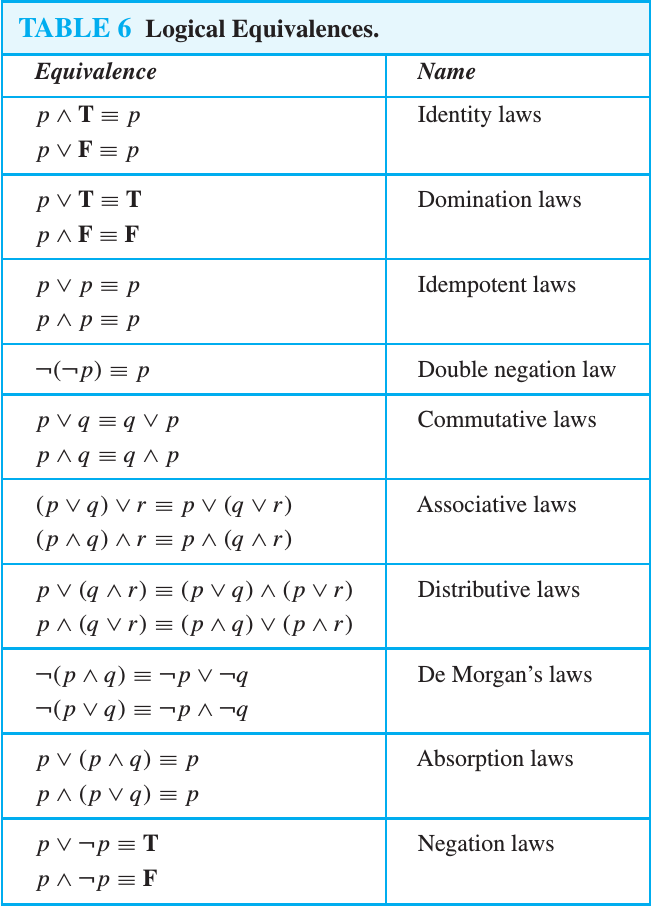
\includegraphics[height=0.8\textheight]{equivalences}
\end{center}
\end{columns}
\end{frame}

\begin{frame}{Sýnt fram á jafngildi}
Við þurfum ekki að nota sanntöflur til að sýna fram á jafngildi. Einföldum ljóta yrðingu:
\begin{align*}
\lnot (p \lor (\lnot p \land q)) &\equiv \lnot p \land \lnot ( \lnot p \land q)\\
&\equiv \lnot p \land (\lnot (\lnot p) \lor \lnot q)\\
&\equiv \lnot p \land (p \lor \lnot q)\\
&\equiv (\lnot p \land p ) \lor (\lnot p \land \lnot q)\\
&\equiv 0 \lor (\lnot p \land \lnot q)\\
&\equiv \lnot p \land \lnot q
\end{align*}
\end{frame}

\begin{frame}{Gerðir sönnunarverkefna}
\begin{itemize}
 \item Oftast erum við að sanna jafngildi eða ``consequence'':
 \item Jafngildi:
 \begin{itemize}
  \item $p \equiv q$, sem þýðir að yrðingin $p$ sé jafngild yrðingunni $q$
  \item $p \equiv q$ er ekki yrðing, en er skylt yrðingunni $p \leftrightarrow q$
 \end{itemize}
 \item Consequence:
 \begin{itemize}
  \item $p \vdash q$, sem þýðir að yrðingin $p$ leiði til yrðingarinnar $q$
  \item $p \vdash q$ er ekki yrðing, en er skylt yrðingunni $p \rightarrow q$
 \end{itemize}
\end{itemize}
\end{frame}


\section{Staðalsnið}

\begin{frame}
\begin{itemize}
 \item Hægt er að setja allar yrðingar fram á stöðluðu formi
 \item Gagnlegt fyrir sannanir
 \begin{itemize}
  \item Sérstaklega tölvusannanir
 \end{itemize}
\end{itemize}
\end{frame}


\begin{frame}{Eð-að staðalsnið}
Fyrir sérhverja yrðingu má finna jafngilda yrðingu á eð-uðu staðalsniði (e. \emph{disjunctive normal form}):
\[
 (a_{11} \land a_{12} \land \ldots \land a_{1r_1} ) \lor (a_{21} \land a_{22} \land \ldots \land a_{2r_2} ) \lor \ldots \lor (a_{n_1} \land a_{n_2} \land \ldots \land a_{nr_n} )
\]

\[
 = \bigvee_{i=1}^n \bigwedge_{j=1}^{r_n}a_{ij}
\]

Þar sem sérhvert $a_{ij}$ er á sniðinu $p$ eða $\lnot p$ fyrir yrðingabreytu $p$.
\end{frame}

\begin{frame}{Og-að staðalsnið}
Fyrir sérhverja yrðingu má finna jafngilda yrðingu á og-uðu staðalsniði (e. \emph{conjunctive normal form}):
\[
 (b_{11} \lor b_{12} \lor \ldots \lor b_{1r_1} ) \land (b_{21} \lor b_{22} \lor \ldots \lor b_{2r_2} ) \land \ldots \land (b_{n_1} \lor b_{n_2} \lor \ldots \lor b_{nr_n} )
\]

\[
 = \bigwedge_{i=1}^n \bigvee_{j=1}^{r_n}b_{ij}
\]

Þar sem sérhvert $a_{ij}$ er á sniðinu $p$ eða $\lnot p$ fyrir yrðingabreytu $p$.
\end{frame}

\begin{frame}{Staðalsnið - dæmi}
Yrðingin
\[
 p \leftrightarrow q
\]
hefur eð-aða staðalsniðið
\[
 (p \land q) \lor (\lnot p \land \lnot q)
\]
og og-aða staðalsniðið
\[
 (p \lor \lnot q) \land (\lnot p \lor q)
\]
\end{frame}

\begin{frame}{Rökstytting til sönnunar}
\begin{itemize}
 \item Rökstytting er notuð til að sanna $p \vdash q$ óbeint fyrir yrðingar $p$ og $q$
 \item Til að beita slíkri aðferð:
 \begin{enumerate}
  \item Forsendan $p$ er sett á og-að staðalsnið
  \begin{itemize}
   \item Hver liður er þá afleiðing af forsendunni
  \end{itemize}
  \item Gerið 1. fyrir \emph{neitunina} af afleiðingunni
  \item Rökstyttingu er beitt á alla liðina sem úr fást þar til mótsögn finnst, sem sýnir að það sé mótsögn að gefa sér að forsendurnar séu sannar og að afleiðingin sé ósönn
 \end{enumerate}
\end{itemize}
\end{frame}


\section{Umsagnir}

\begin{frame}{Umsagnir}
\begin{itemize}
 \item Áður hefur komið fram að ``óræðar'' staðhæfingar á borð við ``$x > 3$'' séu ekki yrðingar
 \item Þessi gerð staðhæfingar felur í sér tvennt:
 \begin{itemize}
  \item Breytuna $x$
  \item Umsögnina (e. \emph{predicate}) ``stærri en 3''
 \end{itemize}
 \item Við getum táknað sanngildi með því að nota yrðingafall (e. \emph{propositional function}) $P(x)$
 \begin{itemize}
  \item $P$ táknar hér umsögnina ``stærri en 3''
 \end{itemize}
 \item Þegar breytunni $x$ hefur verið gefið gildi er staðhæfingin $P(x)$ orðin að yrðingu
\end{itemize}
\end{frame}

\begin{frame}{Dæmi um umsögn}
Látum $P(x)$ áfram tákna ``$x > 3$''. Hvert er sanngildi $P(2)$? \pause

\vspace{0.5cm}
Lausn: Látum $2$ í stað breytunnar $x$ til að fá út yrðingu. Þá er $P(2)$ yrðingin $2 > 3$, sem er ósönn.
\end{frame}

\begin{frame}{Dæmi um umsögn með meira en einni breytu}
Umsagnir geta innihaldið meira en eina breytu. Tákni $Q(x, y)$ staðhæfinguna $x = y + 3$, hvert er þá sanngildi $Q(3, 0)$? \pause
\vspace{0.5cm}

Lausn: $Q(3, 0)$ er yrðingin $3 = 0 + 3$, sem er sönn.
\end{frame}

\section{Magnarar}

\begin{frame}{Magnarar}
\begin{itemize}
 \item Hægt er að búa til yrðingu með yrðingafalli með því að gefa breytu yrðingarinnar gildi
 \item Önnur leið til að búa til yrðingu úr yrðingafalli er að nota magnara (e. \emph{quantifier})
 \item Stærðfræðin sem snýr að umsögnum og mögnurum kallast umsagnarökfræði (e. \emph{predicate calculus})
\end{itemize}
\end{frame}

\begin{frame}{Magnarar og óðöl}
\begin{itemize}
 \item Við munum skoða tvær gerðir magnara:
 \begin{itemize}
  \item Almagnarinn (e. \emph{the universal quantifier}) segir að umsögn sé sönn fyrir öll möguleg gildi í menginu sem verið er að skoða
  \begin{itemize}
   \item Almagnarinn er táknaður með $\forall$
  \end{itemize}
  \item Tilvistarmagnarinn (e. \emph{the existance quantifier}) segir að umsögn sé sönn fyrir að minnsta kosti eitt mögulegt gildi í menginu sem verið er að skoða
  \begin{itemize}
   \item Tilvistarmagnarinn er táknaður með $\exists$
  \end{itemize}
 \end{itemize}
 \item ``Mengi sem um ræðir'' er kallað óðal (e. \emph{domain})
\end{itemize}
\end{frame}

\begin{frame}{Magnarar og óðöl}
\begin{itemize}
 \item Fyrir óðal allra lífvera getum við skilgreint yrðingaföll:
 \begin{itemize}
  \item $M(x) = $ ``$x$ er mannvera''
  \item $D(x) = $ ``$x$ er dauðleg''
 \end{itemize}
 \item Þá getum við notað magnara til að smíða yrðingar:
 \begin{itemize}
  \item $\exists x: D(x)$ (til er dauðleg lífvera)
  \item $\exists x: M(x) \land D(x)$ (til er dauðleg mannvera) \pause
  \item $\forall x: M(x) \to D(x)$ (allar mannverur eru dauðlegar)
 \end{itemize}
\end{itemize}
\end{frame}

\begin{frame}{Reglur De Morgans fyrir magnara}
Neitun tilvistar breytist í almögnun:
\[
 \lnot \exists x: P(x) \equiv \forall x: \lnot P(x)
\]
Neitun alvistar breytist í tilvist:
\[
 \lnot \forall x: P(x) \equiv \exists x: \lnot P(x)
\]
\end{frame}

\begin{frame}{Dæmi með mögnurum}
\begin{itemize}
 \item Dæmi frá Lewis Caroll (Lísa í Undralandi)
 \item Gefið er:
 \begin{itemize}
  \item ``Öll ljón eru grimm''
  \item ``Sum ljón drekka ekki kaffi''
 \end{itemize}
 \item Viljum sanna:
 \begin{itemize}
  \item ``Sumar grimmar skepnur drekka ekki kaffi''
 \end{itemize}
 \item Túlkum:
 \begin{itemize}
  \item Óðalið er allar skepnur
  \item Táknum ``$x$ er ljón'' með $L(x)$
  \item Táknum ``$x$ er grimm skepna'' með $G(x)$
  \item Táknum ``$x$ drekkur kaffi'' með $K(x)$
 \end{itemize}
\end{itemize}
\end{frame}

\begin{frame}{Framsetning með mögnurum}
\begin{itemize}
 \item Forsendur:
 \begin{itemize}
  \item $\forall x: L(x) \to G(x)$ (öll ljón eru grimm)
  \item $\exists x: L(x) \land \lnot K(x)$ (til er ljón sem ekki drekkur kaffi)
 \end{itemize}
 \item Afleiðing:
 \begin{itemize}
  \item $\exists x: G(x) \land \lnot K(x)$ (til er grimm skepna sem ekki drekkur kaffi)
 \end{itemize}
 \item Hægt er að sýna fram á þessi tengsl með rökstyttingu
\end{itemize}
\end{frame}

\begin{frame}<presentation:0>{Sönnun með mögnurum}
\begin{itemize}
 \item Umbreytum forsendunum til að þær séu á sama sniði:
 \begin{itemize}
  \item $\forall x: L(x) \to G(x)$ verður $ \forall x:(\lnot L(x) \lor G(x))$
  \item $\exists x: L(x) \land \lnot K(x)$ verður $L(c) \land \lnot K(c)$ með breytuskiptum, þar sem $c$ er eitthvert ljón sem ekki drekkur kaffi
 \end{itemize}
 \item Neitum nú afleiðingunni, og umbreytum:
 \begin{itemize}
  \item $\lnot \exists x: G(x) \land \lnot K(x)$ verður $\forall x: \lnot (G(x) \land \lnot K(x))$ með De Morgan fyrir magnara
  \item sem verður $\forall x: \lnot G(x) \lor \lnot \lnot K(x)$ með De Morgan fyrir neitun og-unar
  \item sem verður $\forall x: (\lnot G(x) \lor K(x))$ með neitun neitunar (allar skepnur eru annaðhvort ekki grimmar eða þær drekka kaffi)
 \end{itemize}
\end{itemize}
\end{frame}

\begin{frame}{Næst}
Í næsta tíma: Mengi og mengjaaðgerðir (kaflar 2.1 og 2.2)
\end{frame}


\end{document}
